\documentclass{article}
\usepackage[utf8]{inputenc}
\usepackage[margin=1in]{geometry}
\usepackage{soul,color}
\usepackage{amsfonts, amsmath}
\usepackage{bbm}
\usepackage{enumitem}
\usepackage[nobreak=true]{mdframed}
\usepackage{amssymb}
\usepackage{graphicx}

\newcommand{\solution}{\textbf{Solution: }}
\newcommand{\N}{\mathcal{N}}
% \newcommand{\Pbf}{\textbf{P}}
\newcommand{\R}{\mathbb{R}}
\newcommand{\E}{\mathbb{E}}
\newcommand{\Var}{\text{Var}}
\newcommand{\Cov}{\text{Cov}}
\newcommand{\Ell}{\mathcal{L}}
\DeclareMathOperator*{\argmin}{argmin}

\usepackage[utf8]{inputenc}

% Default fixed font does not support bold face
\DeclareFixedFont{\ttb}{T1}{txtt}{bx}{n}{8} % for bold
\DeclareFixedFont{\ttm}{T1}{txtt}{m}{n}{8}  % for normal

% Custom colors
\usepackage{color}
\definecolor{deepblue}{rgb}{0,0,0.5}
\definecolor{deepred}{rgb}{0.6,0,0}
\definecolor{deepgreen}{rgb}{0,0.5,0}

\usepackage{listings}

% Python style for highlighting
\newcommand\pythonstyle{\lstset{
language=Python,
basicstyle=\ttfamily\footnotesize,
otherkeywords={self},             % Add keywords here
keywordstyle=\ttb\color{deepblue},
emph={MyClass,__init__},          % Custom highlighting
emphstyle=\ttb\color{deepred},    % Custom highlighting style
stringstyle=\color{deepgreen},
frame=tb,                         % Any extra options here
showstringspaces=false           % 
}}


% Python environment
\lstnewenvironment{python}[1][]
{
\pythonstyle
\lstset{#1}
}
{}

% Python for external files
\newcommand\pythonexternal[2][]{{
\pythonstyle
\lstinputlisting[#1]{#2}}}

% Python for inline
\newcommand\pythoninline[1]{{\pythonstyle\lstinline!#1!}}

\title{CS189, HW4: Regression}
\author{ Completed by: Matthew Wu}
% \date{January 2017}
\date{}

\begin{document}

\maketitle

\subsection*{1. Logistic Regression with Newton's Method}
\begin{enumerate}[label=\arabic*)]
\item
$$J(w)=\lambda |w|_2^2-\sum_{i=1}^4\bigg(y_i \ln s_i+(1-y_i)\ln(1-s_i)\bigg)$$
$$\frac{\partial}{\partial w} \lambda |w|_2^2 = \frac{\partial}{\partial w} \lambda w^\top w=2\lambda w$$
$$\nabla_wJ=2\lambda w - \sum_{i=1}^4(y_i-s_i)X_i$$
$$\nabla_wJ=2\lambda w - X^\top (y-s)$$
%$$\frac{\partial J_i}{\partial w}=-(y_i\ln s_i +(1-y_i)\ln(1-s_i))$$
%$$=-(y_i \frac{1}{s_i}s_i(1-s_i)X_i-(1-y_i)\frac{1}{1-s_i}s_i(1-s_i)X_i)$$
%$$=-(y_i\frac{1}{s_i}-(1-y_i)\frac{1}{1-s_i})s_i(1-s_i)X_i$$
%$$=-(y_i(1-s_i)-(1-y_i)s_i)X_i$$
%$$=-(y_i-s_i)X_i$$
%$$\triangledown J_w=2w-\sum_{i=1}^n(y_i-s_i)X_i=2w$$
\item
$$\nabla_w^2J=2\lambda I + \sum_{i=1}^4 s_i(1-s_i)X_iX_i^\top$$
$$\nabla_w^2J=2\lambda I + X^\top\Omega X\text{, where }\Omega=
\begin{bmatrix}
s_1(1-s_1) & 0 & 0 & 0\\
0 & s_2(1-s_2) & 0 & 0\\
0 & 0 & s_3(1-s_3) & 0\\
0 & 0 & 0 & s_4(1-s_4)
\end{bmatrix}$$
\item
$$w^{(n+1)}=w^{(n)}+H^{-1}\nabla_wJ$$
$$=w^{(n)}-(2\lambda I + X^\top \Omega X)^{-1}(2\lambda w - X^\top(y-s))$$
\item
Code for calculations provided in the appendix
\begin{enumerate}[label=\alph*)]
\item $s^{(0)}=\begin{bmatrix}0.95257413 & 0.73105858 & 0.73105858 & 0.26894142\end{bmatrix}^T$
\item $w^{(1)}=\begin{bmatrix}-0.38676399 & 1.40431761 & -2.28417115\end{bmatrix}^T$
\item $s^{(1)}=\begin{bmatrix}0.87311451 & 0.82375785 & 0.29320813 & 0.21983683\end{bmatrix}^T$
\item $w^{(2)}=\begin{bmatrix}-0.51222668 & 1.45272677 & -2.16271799\end{bmatrix}^T$
\end{enumerate}
\end{enumerate}


\newpage


\subsection*{2. $\ell_1$ and $\ell_2$ Regularization}
\begin{enumerate}[label=\arabic*)]
\item
$$J(w)=|Xw-y|^2+\lambda \lVert w \rVert_{\ell_1}$$
$$J(w)=(Xw-y)^T(Xw-y)+\sum_{i=1}^d \lambda w_i$$
$$J(w)=y^Ty+w^TX^TXw - 2y^TXw + \sum_{i=1}^d \lambda |w_i|$$
$$J(w)=y^Ty+\sum_{i=1}^d nw_i^2-2y^TX_{*i}w_i+\lambda |w_i|$$
$$g(y) = y^Ty, \quad f(\cdot) = nw_i^2-2y^TX_{*i}w_i+\lambda |w_i|$$
\item If $w^*_i>0$, then
$$\frac{\partial J}{\partial w^*_i}=2nw^*_i-2y^TX_{*i}+\lambda=0$$
$$w^*_i=\frac{2y^TX_{*i}-\lambda}{2n}$$
\item If $w^*_i<0$, then
$$\frac{\partial J}{\partial w^*_i}=2nw^*_i-2y^TX_{*i}-\lambda=0$$
$$w^*_i=\frac{2y^TX_{*i}+\lambda}{2n}$$
\item
Assume that $w^*_i$ is 0. Then the neither the equation where $w^*_i$ is positive nor the equation where $w^*_i$ is negative can be true. Thus, we have $\frac{2y^TX_{*i}-\lambda}{2n} \leq 0$, and $\frac{2y^TX_{*i}+\lambda}{2n} \geq 0$.
$$\frac{2y^TX_{*i}-\lambda}{2n} \leq 0 \Rightarrow 2y^TX_{*i} \leq \lambda$$
$$\frac{2y^TX_{*i}+\lambda}{2n} \geq 0 \Rightarrow -2y^TX_{*i} \leq \lambda$$

Suppose that $\lambda \geq |2y^TX_{*i}|$, then $w^*_i>0$ and we set the gradient equal to 0, then we have\\ $w^*_i=\frac{2y^TX_{*i}-\lambda}{2n} \leq 0$, so $w^*_i$ can't be positive. Likewise, if $w^*_i < 0$ and we set the gradient equal to 0, we have $w^*_i=\frac{2y^TX_{*i}+\lambda}{2n} \geq 0$, so $w^*_i$ can't be negative. Therefore, if $\lambda \geq |2y^TX_{*i}|$, then $w^*_i$ must be 0.

Therefore, $w^*_i$ if and only if $\lambda \geq |2y^TX_{*i}|$.

\item $$f(\cdot)=nw_i^2-2y^TX_{*i}w_i+\lambda w_i^2$$
$$\frac{\partial J}{\partial w^*_i} = 2nw_i - 2y^TX_{*i} + 2\lambda w_i=0$$
$$w^*_i=0 \Rightarrow 2y^TX_{*i}=0$$
Now $w^*_i=0$ only if $2y^TX_{*i}$ is exactly 0, as opposed to being able to make a weight 0 with a large enough $\lambda$.
\end{enumerate}


\newpage
\subsection*{3. Regression and Dual Solution}
\begin{enumerate}[label=\alph*)]
\item $$\nabla |w|^4=(w^Tw)^2=2(w^Tw)2w=(4w^Tw)w$$
$$\nabla_w |Xw-y|^4=((Xw-y)^T(Xw-y))^2=2(Xw-y)^T(Xw-y)2X^T(Xw-y)$$
$$=4(Xw-y)^T(Xw-y)X^T(Xw-y)$$

\item
To prove $w^*$ is unique, we can show that the function is convex by proving the hessian is positive definite.
$$\nabla_w^2|Xw-y|^4+\lambda|w|^2=\nabla_w^2|Xw-y|^4 + \nabla_w^2 \lambda|w|^2$$
Let $g(w)=|Xw-y|^2$, $f(x)=x^2$, and $h(w)=f(g(w))$ so
$$\nabla^2h(w)=f''(g(w))\nabla g(w)\nabla g(w)^T + f'(g(w))\nabla^2g(w)$$
$$\nabla g(w)=2X^T(Xw-y) \qquad \nabla^2g(w)=2X^TX$$
$$\nabla_w^2|Xw-y|^4=8 X^T(Xw-y)(X^T(Xw-y))^T+4|Xw-y|^2X^TX$$
Any matrix that can be written in the form $UU^T$ is positive semidefinite, and $8$ and $4|Xw-y|^2$ are nonnegative scalars, so $\nabla_w^2|Xw-y|^4$ is positive semidefinite.
$$\nabla_w^2\lambda|w|^2 = 2\lambda I\text{, which is positive definite.}$$
Since $\nabla_w^2|Xw-y|^4$ is positive semidefinite, and $\nabla_w^2\lambda|w|^2$ is positive definite, $\nabla_w^2|Xw-y|^4+\lambda|w|^2$ is positive definite, which is sufficient to show $w^*$ is unique.
$$\nabla_w |Xw-y|^4+\lambda|w|^2=4(Xw-y)^T(Xw-y)X^T(Xw-y)+2\lambda w=0$$
$$\text{Let }(Xw-y)^T(Xw-y)=c$$
$$4cX^T(Xw-y)+2\lambda w=0$$
$$2\lambda w = 4cX^T(y-Xw)$$
$$w^*=X^Ta=\sum_{i=1}^na_iX_i \text{, where}$$
$$a=\frac{2}{\lambda}c(y-Xw^*)=\frac{2}{\lambda}(Xw^*-y)^T(Xw^*-y)(y-Xw^*)$$
\item
$$w^*=\argmin_{w\in \R^d} \frac{1}{n}\sum_{i=1}^nL(w^TX_i,y_i)+\lambda|w|^2=\argmin_{w\in \R^d}\lambda|w|^2+\frac{1}{n}\sum_{i=1}^nL(w^TX_i,y_i)$$
$$\nabla_w\lambda|w|^2+\frac{1}{n}\sum_{i=1}^nL(w^TX_i,y_i)=2\lambda w+\frac{1}{n}\sum_{i=1}^n \nabla_w(L(w^TX_i,y_i))X_i$$
$$w=-\frac{1}{2\lambda n}\sum_{i=1}^n\nabla_w(L(w^TX_i,y_i))X_i=X^Ta\text{, where }a=-\frac{1}{2\lambda n}\nabla_w(L(w^TX_i,y_i))$$
Therefore the optimal value $w^*$ is a linear combination of the samples of $X$ regardless of whether or not it is convex. However, the optimal solution in the case where the loss function isn't convex, $w^*$ may not be unique.
\end{enumerate}

\newpage
\subsection*{4. Franzia Classification + Logistic Regression = Party!}
Prior to training the classifier, I shuffle the training data, add a bias feature, and normalize across the columns of all samples (including the test samples), and set aside 1000 samples for validation.

\begin{enumerate}[label=\arabic*)]
\item
Let $X$ be a normalized, $n \times d$ design matrix, and $y$ be an $n$-vector with $y_1, y_2, \dots, y_n \in \{0, 1\}$. We want to solve the following expression:
$$\argmin_{w \in \R^d}J(w)=\lambda |w|^2-\sum_{i=1}^n\bigg(y_i\ln s(X_i^Tw)+(1-y_i)\ln(1-s(X_i^Tw))\bigg)$$
$$\nabla_{w}J=2\lambda w - X^T(y-s(Xw))$$
$$\text{batch update: } w \leftarrow w + \epsilon(X^T(y-s(Xw))-2\lambda w)$$
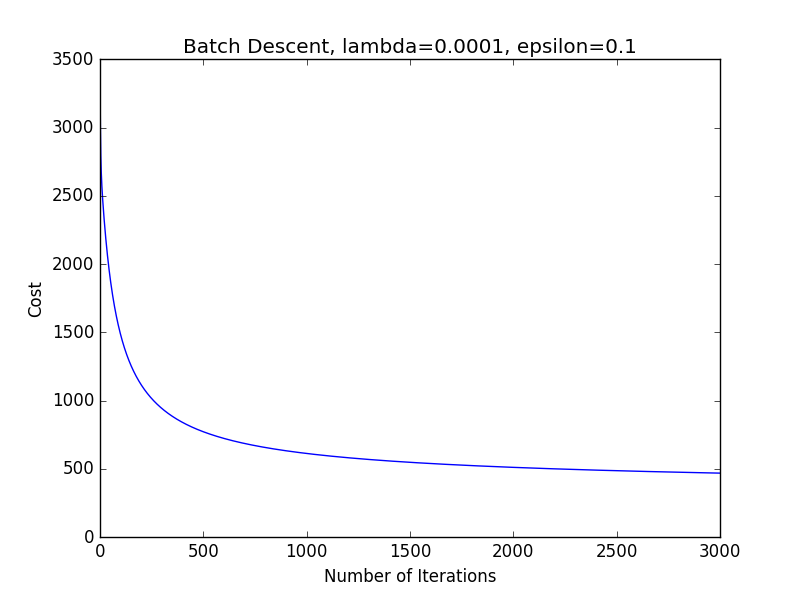
\includegraphics[scale=.6]{images/batch.png}

The cost function gets to a bit below 500, and still hasn't quite converged after 3000 iterations with $\epsilon=0.1$.

\newpage
\item
$$\nabla_wJ = 2\lambda w - X^T(y-s(Xw))$$
$$\text{stochastic update: } w \leftarrow w + \epsilon((y_i-s(X_i^Tw))X_i - 2\lambda w)$$
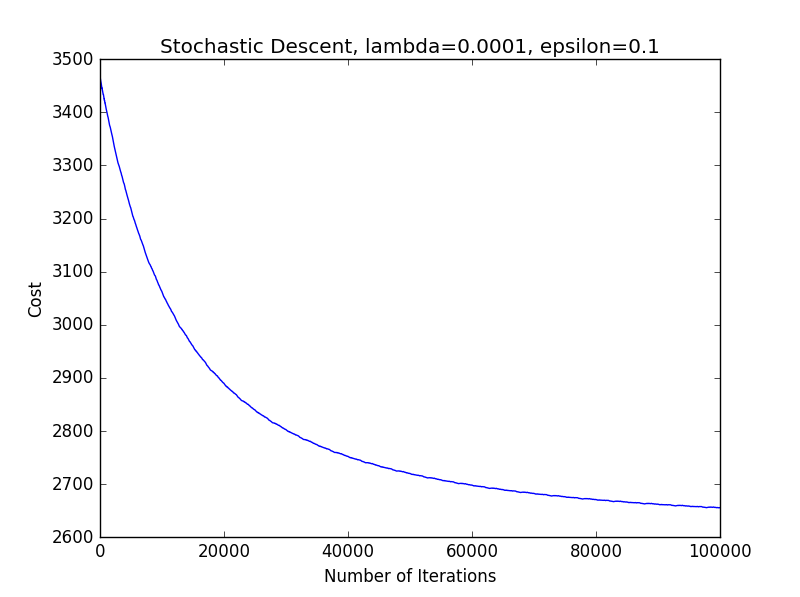
\includegraphics[scale=.6]{images/stoch.png}

Although the cost function hasn't converged, it has nearly converged and the cost is still well over 2600, no where near the 500 produced by batch descent. Stochastic gradient descent is faster to calculate, but it doesn't achieve nearly the same level of accuracy as batch descent in practice, because there is more noise in one sample than when averaging across all samples.

\item
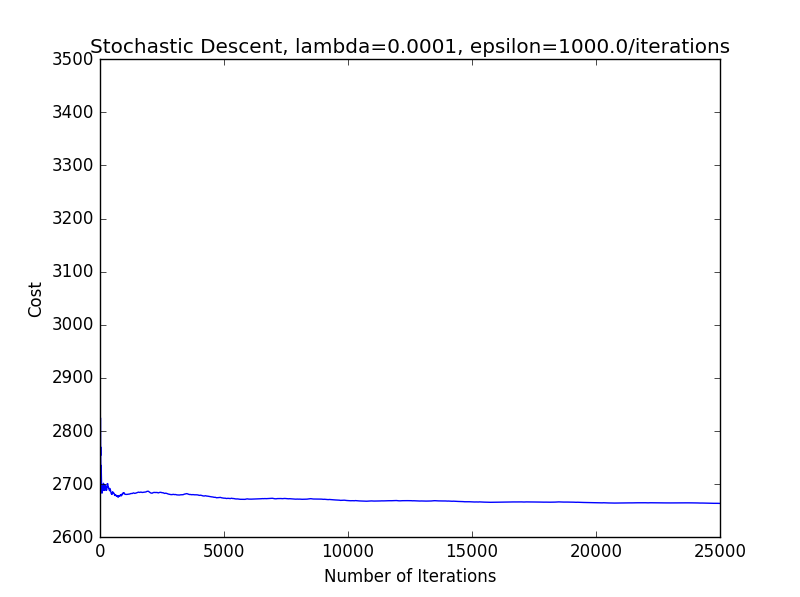
\includegraphics[scale=.6]{images/stoch_vary.png}

Using an $\epsilon$ that varies directly with time converges the cost function far more quickly (less than $\frac{1}{4}$ the iterations) than using a constant $\epsilon$, making it a better strategy for training the classifier.

\item
For the Kaggle submission, I used batch gradient descent, varying epsilon from $0.2$ to $0.1$ linearly, and increased the number of iterations to $4000$. I experimented with different values of $\lambda$ and $\epsilon$ for batch gradient descent, observing both the cost of the training data and the error rate of classification of the validation set. The value of $\lambda$ I settled on was $\lambda=.0001$, and the value of $\epsilon$ was determined from observing how the cost function converged, and varying $\epsilon$, as it helps the cost function converge faster as noted in part 3.


My Kaggle display name is Commendable Fennel, and my best submission had an accuracy rate of 0.97984.

\end{enumerate}

\newpage
\section*{5. Real World Spam Classification}

\quad \, Since we have a quadratic model, ideally we want all the emails that are likely to classified as spam for this particular feature to all be close to the same value. Since we're limited to a quadratic model, creating a function that sends messages sent near midnight to close to the same value will give the classier the best chance at isolating these emails.\\

If we store the number of milliseconds since the previous midnight, that means that this particular feature should attempt to classify messages with a features near 0 or features near 86,400,000 as spam, and messages in the middle of those as not spam. However, since we're limited to a quadratic, our quadratic will tend to classify messages that are a few hours before or after midnight as spam as well, since there will be a sharp increase towards more likely to be spam towards 0 and 86,400,000.\\

If we instead choose to map the feature to the number of milliseconds to the closest midnight, then our classifier will be much better at fitting to this feature. When trying to classify this feature, the quadratic will form a parabola with an extremum at $0$, which will be able to classify emails sent near that time as spam, with a gradual decrease towards being less likely to be spam, as opposed to the sharp shape from the previous featurization.

\newpage
\section*{Appendix}
The following code was used for newton's method in question 1:

\begin{python}
import numpy as np

X = np.array(
    [[0, 3, 1],
    [1, 3, 1],
    [0, 1, 1],
    [1, 1, 1]]
    )
y = np.array([[1], [1], [0], [0]])

lam = 0.07

w = np.array([[-2], [1], [0]])

def sigmoid(x):
    return 1/(1+np.exp(-x))

for i in range(2):
    s = []
    for j in range(4):
        s.append(sigmoid(np.dot(X[j], w)))
    s = np.array(s).reshape(4, 1)
    print("s" + str(i) + " = " + str(np.transpose(s)))
    omega = np.array(
        [[s[0][0]*(1-s[0][0]), 0, 0, 0],
        [0, s[1][0]*(1-s[1][0]), 0, 0],
        [0, 0, s[2][0]*(1-s[2][0]), 0],
        [0, 0, 0, s[3][0]*(1-s[3][0])]])
    A = np.linalg.inv(np.add(2*lam*np.eye(3), np.dot(np.transpose(X), np.dot(omega, X))))
    B = np.subtract(2*lam*w, np.dot(np.transpose(X), y-s))
    w = w - np.dot(A, B)
    print("w" + str(i+1) + " = " + str(np.transpose(w)))
\end{python}
\vskip 1.5in
\begin{python}
         __
        /  \
       / ..|\
      (_\  |_)
      /  \@`
     /     \
_   /  `   |
\\_/  \ | _\
 \    /_|| \\_
  \____)|_) \_)
\end{python}

\newpage

The following code was used for plotting and training the wine classifier:

\begin{python}    
import numpy as np
import scipy.io
import matplotlib.pyplot as plt
import csv
import sys

traindatafilename = "data"
data = scipy.io.loadmat(traindatafilename)

#Load and shuffle data sets
traindata = data['X']
NUM_FEATURES = traindata.shape[1]
NUM_SAMPLES = traindata.shape[0]
testdata = data['X_test']
labels = data['y']

temp = np.hstack((traindata, labels))
np.random.shuffle(temp)
X = temp[:,:NUM_FEATURES]

#Add bias term and normalize across all samples
tempmerge = np.vstack((X, testdata))
tempmerge = np.hstack((tempmerge, np.ones(6497).reshape(6497, 1)))
tempmerge = tempmerge / np.linalg.norm(tempmerge, axis=0)[np.newaxis, :]
X = tempmerge[:NUM_SAMPLES]
testdata = tempmerge[NUM_SAMPLES:]

y = temp[:,NUM_FEATURES:]

NUM_FEATURES += 1

TRAINING_SIZE = 5000
VALIDATION_SIZE = NUM_SAMPLES - TRAINING_SIZE

X_train = X[:TRAINING_SIZE]
y_train = y[:TRAINING_SIZE]

X_validation = X[TRAINING_SIZE:]
y_validation = y[TRAINING_SIZE:]

LAMBDA = .0001

def sigmoid(Xi, w):
    return 1 / (1 + np.exp(-np.dot(Xi.transpose(), w)))

def cost(XX, yy, w):
    norm_cost = LAMBDA * np.dot(w.transpose(), w)
    samples_cost = 0
    for i in range(XX.shape[0]):
        Xi, y_i = XX[i].transpose(), yy[i]
        if y_i == 1:
            samples_cost += np.log(sigmoid(Xi, w))
        else:
            samples_cost += np.log(1-sigmoid(Xi, w))
    return float(norm_cost - samples_cost)

def classify(XX, w):
    """Returns list of classified samples based on w"""
    s = [sigmoid(XX[i], w) for i in range(XX.shape[0])]
    p = [int(np.round(i)) for i in s]
    return p

def plot_batch():
    EPSILON = .1
    training_cost_list = []
    validation_cost_list = []
    num_iteration = []
    w = X_train[:1].transpose() #Initialize w
    training_cost_list.append(cost(X_train, y_train, w))
    validation_cost_list.append(cost(X_validation, y_validation, w))
    num_iteration.append(0)
    MAX_ITERATIONS = 3000
    for iteration in range(1, MAX_ITERATIONS + 1):
        s_vector = []
        for i in range(TRAINING_SIZE):
            Xi = X_train[i].transpose()
            s_vector.append(sigmoid(Xi, w))
        s_vector = np.array(s_vector).reshape(TRAINING_SIZE, 1)
        w = w + EPSILON * (np.dot(X_train.transpose(), y_train - s_vector)
            - 2 * LAMBDA * w)
        if iteration % 1 == 0:
            num_iteration.append(iteration)
            training_cost_list.append(cost(X_train, y_train, w))
            validation_cost_list.append(cost(X_validation, y_validation, w))
    print("Final training cost: " + str(training_cost_list[-1]))
    print("Final validation cost: " + str(validation_cost_list[-1]))

    val_guesses = classify(X_validation, w)
    total = 0
    wrong = 0
    for i in range(len(val_guesses)):
        if val_guesses[i] != y_validation[i]:
            wrong += 1
        total += 1
    print("Error Rate: " + str(wrong/total))
    sys.stdout.flush()

    plt.figure()
    plt.plot(num_iteration, training_cost_list)
    plt.title("Batch Descent, lambda="
        + str(LAMBDA) + ", epsilon=" + str(EPSILON))
    plt.ylabel("Cost")
    plt.xlabel("Number of Iterations")
    plt.figure()
    plt.plot(num_iteration, validation_cost_list)
    plt.title("Batch Descent Validation, lambda="
        + str(LAMBDA) + ", epsilon=" + str(EPSILON))
    plt.ylabel("Cost")
    plt.xlabel("Number of Iterations")
    plt.show()

def plot_stochastic(use_varying_epsilon=False):
    EPSILON = .1
    MULTIPLIER = 10000
    epsilon = EPSILON
    training_cost_list = []
    num_iteration = []
    w = X_train[:1].transpose() #Initialize w
    training_cost_list.append(cost(X_train, y_train, w))
    num_iteration.append(0)
    MAX_ITERATIONS = 20*TRAINING_SIZE
    for iteration in range(1, MAX_ITERATIONS + 1):
        i = iteration % TRAINING_SIZE
        Xi = X_train[i].reshape(NUM_FEATURES, 1)
        c = y_train[i] - sigmoid(Xi, w)
        if use_varying_epsilon:
            epsilon = EPSILON * MULTIPLIER / iteration
        w = w + epsilon * (c * Xi - 2 * LAMBDA * w)
        if iteration < 100 or iteration % 5 == 0 and iteration < 1000\
            or iteration % 50 == 0:
            num_iteration.append(iteration)
            training_cost_list.append(cost(X_train, y_train, w))
    print("Final training cost: " + str(training_cost_list[-1]))
    print("Final validation cost: " + str(cost(X_validation, y_validation, w)))
    val_guesses = classify(X_validation, w)
    total = 0
    wrong = 0
    for i in range(len(val_guesses)):
        if val_guesses[i] != y_validation[i]:
            wrong += 1
        total += 1
    print("Error Rate: " + str(wrong/total))
    sys.stdout.flush()

    if use_varying_epsilon:
        epsilon = EPSILON * MULTIPLIER

    plt.figure()
    plt.plot(num_iteration, training_cost_list)

    string = "Stochastic Descent, lambda="
    string += str(LAMBDA) + ", epsilon=" + str(epsilon)
    if use_varying_epsilon:
        string += "/iterations"
    plt.title(string)
    plt.ylabel("Cost")
    plt.xlabel("Number of Iterations")
    plt.show()

def classify_batch():
    global testdata
    EPSILON = .1
    num_iteration = []
    w = X[:1].transpose() #Initialize w
    num_iteration.append(0)
    MAX_ITERATIONS = 4000
    for iteration in range(1, MAX_ITERATIONS + 1):
        s_vector = []
        for i in range(TRAINING_SIZE):
            Xi = X[i].transpose()
            s_vector.append(sigmoid(Xi, w))
        s_vector = np.array(s_vector).reshape(TRAINING_SIZE, 1)
        eps = (2 - iteration / MAX_ITERATIONS / 2) * EPSILON
        w = w + eps * (np.dot(X_train.transpose(), y_train - s_vector)
            - 2 * LAMBDA * w)
        if iteration % 1 == 0:
            num_iteration.append(iteration)
    testdata = testdata / np.linalg.norm(testdata, axis=1)[:, np.newaxis]
    guesses = classify(testdata, w)
    with open('submission_1.csv', 'w', newline='') as csvfile:
        writer = csv.writer(csvfile)
        writer.writerow(['Id', 'Category'])
        i = 0
        for g in guesses:
            writer.writerow([i, g])
            i += 1

#plot_batch()
#plot_stochastic(use_varying_epsilon=False)
#plot_stochastic(use_varying_epsilon=True)
#classify_batch()
\end{python}
\end{document}